\chapter{Introduction}

\section{Motivation}
\gls{ic} is a faculty of \gls{kmitl}. 
IC has been up and running well for 6 years.
About 25 employees are working here. %TODO add number of students, lecturers
Their main objective is to provide educational services to students. 
Right now, they have a trouble with paper clutter. 
Even though they have organized documents into categories. 
The organization takes countless hours to organize, store, and retrieve documents.
This problem hinders employee's productivity when they need to retrieve many documents. 
Another problem is losing track of document during its workflow execution. 
A workflow is a series of repeatable steps performed in a sequential manner to reach a goal.
Each type of workflow usually associates with a set of actions. 
A person who receive a document will execute some actions depending on their responsibility.
They have to execute them sequentially. 
Some workflows are very complicated and very difficult to keep track of.

IC would like to prevent these problems before it goes out of control. 
Our proposed solution is to manage, store, and retrieve documents digitally using a computer software.
The employee will use less time to search and be less error-prone.
We will create a system that provide ability to search and to track documents.
We are working on \dms.
Because we want to provide a system to manage documents within IC.
Once we do, IC can manage and track documents more efficient, thus, increase organization's productivity.

\section{Objective}
% list of our primary objectives
Our primary objectives are
\begin{enumerate}
\item To get the workflow model and to track document's current state during its workflow execution. 
\item To report other related or dependent documents required by its originator.
\item To store and retrieve digital documents that complete its workflow from one centralized IC's server.
\end{enumerate}

\section{Scope}
We are going to develop a web-based application hosted on an IC's server.
Only people within IC and granted external users can access the system.
To be specific, there are 4 types of users.
\begin{enumerate}
\item IC's staffs.
%TODO list all employee's position who invovled in this system
\item KMITL lecturers who is assigned to IC.
\item Stdents who is currently enroll in IC, KMITL.
\item External users who is allowed to access the system by IC.
\end{enumerate}

The system have to manage only document distributed officially by IC.
This also includes other attachments from external sources given that IC requires them.
No personal document involved.

\section{Project plan}
The project starts at August 18th, 2015.
We expect to deliver it on March 25th, 2016.
For our project planing, we divide our work into 4 phases.
%TODO descibe them
\begin{enumerate}
\item Plan and research (18/08/15 -- 30/10/15) \hfill \\

\item Design and architecture (29/09/15 -- 23/11/15) \hfill \\

\item System implementation (7/12/15 -- 22/02/16) \hfill \\

\item Testing (19/02/16 -- 07/03/16) \hfill \\

\end{enumerate}

\begin{landscape}
\begin{figure}
\centering
\caption{Project's schedule shown as Gantt chart}
\label{fig:project-schedule}
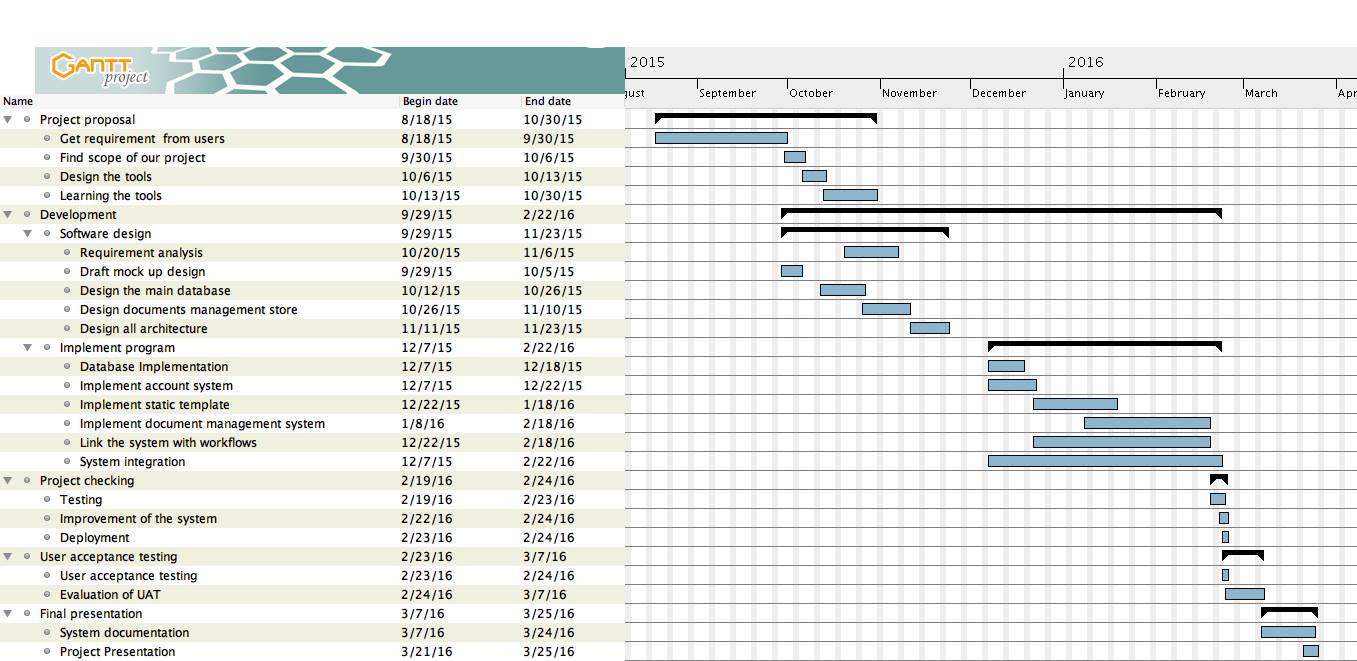
\includegraphics[scale=0.45]{res/project_plan}
\end{figure}
\end{landscape}